\label{sec:preliminary_experiments}

As discussed in the previous chapter, the optimizer’s behavior is driven by indices, cost settings, strategy settings, and its general perception of the data distribution. Database systems come with basic configurations tuned for broad compatibility rather than optimal performance. As the default parameters may be unsuitable in some scenarios, database systems allow disabling different strategy settings on a per-query or permanent basis to dissuade the optimizer from going down an unproductive path.

To analyze the impact of enabling or disabling strategy settings on query runtime, we set up a scenario that considers an out-of-the-box PostgreSQL~\citep{PostGreSQL} server instance and two different queries from the Join Order Benchmark (\gls{job})~\citep{JOB} workload, which is described in further detaile in Section \ref{sec:workloads}. First, each query is executed without any strategy restrictions, in which all settings are enabled, and then executed with strategies that tend to be costly disabled, establishing a comparison among these settings in the end.

\begin{figure}[H]
  \begin{subfigure}[t]{0.5\textwidth}
    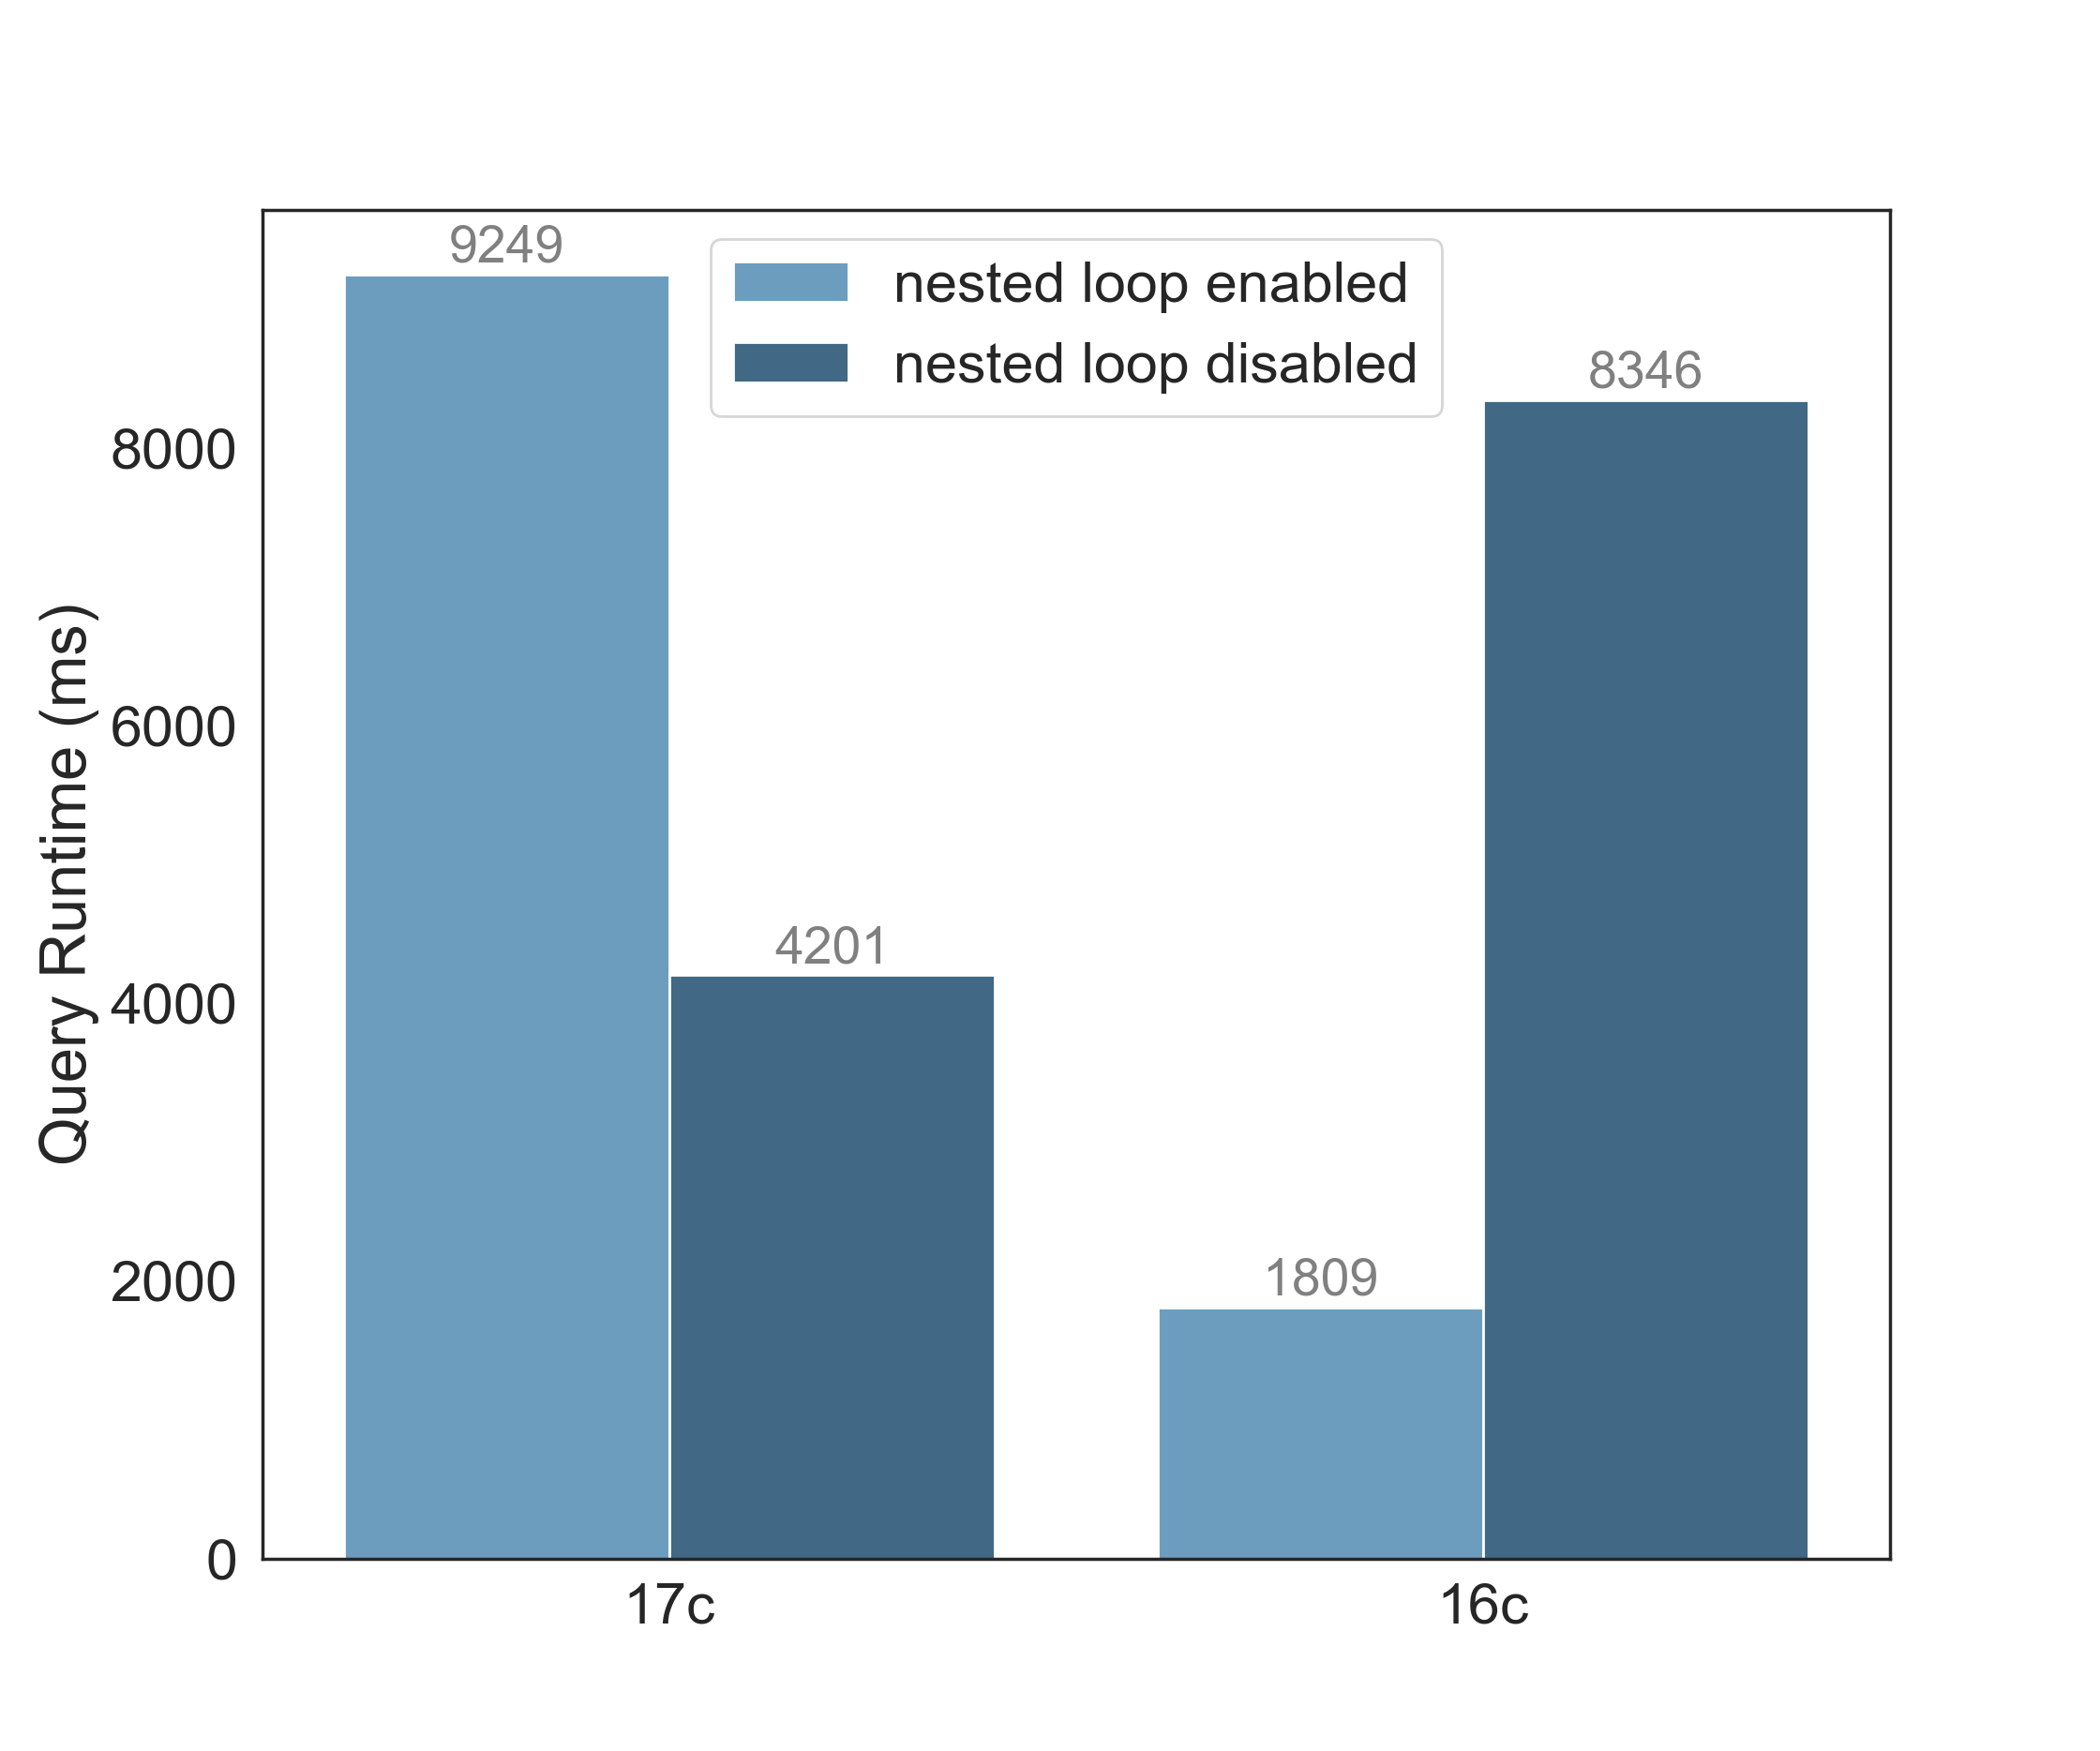
\includegraphics[width=\textwidth]{img/solution/nested_loop_experiment.png}
    \label{fig-a}
  \end{subfigure}\hfill
  \begin{subfigure}[t]{0.5\textwidth}
    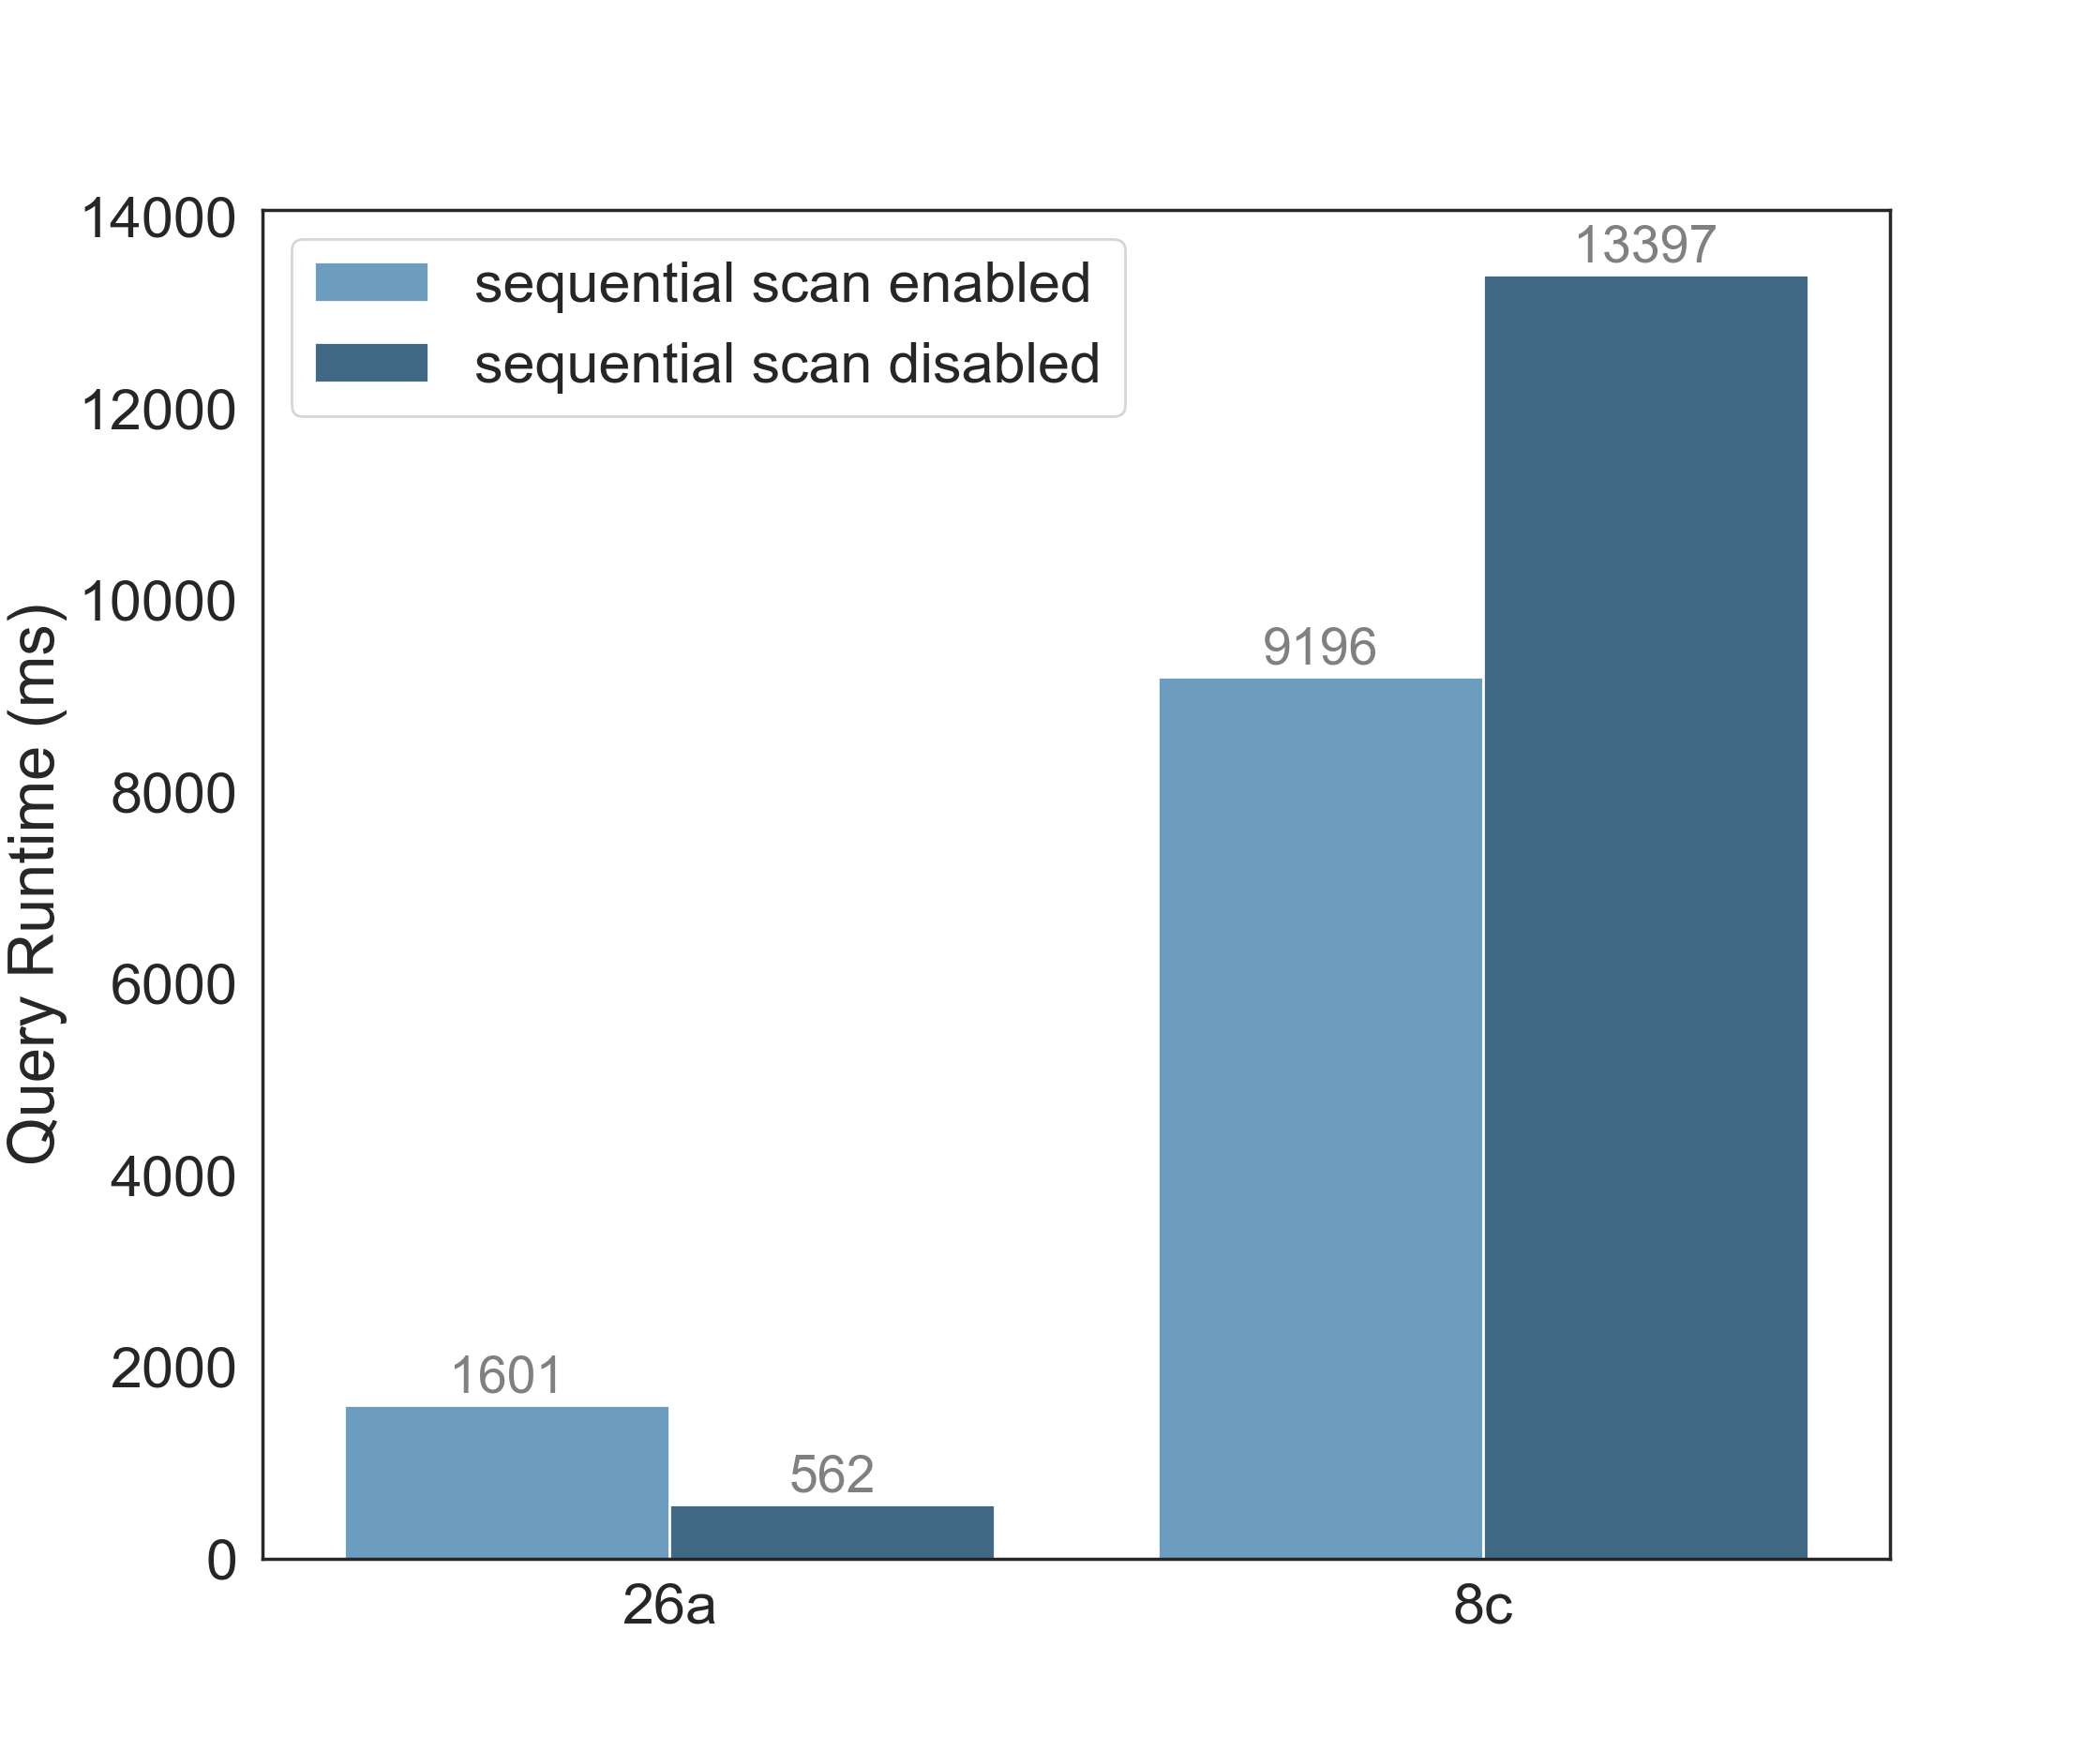
\includegraphics[width=\textwidth]{img/solution/sequential_scan_experiment.png}
    \label{fig-b}
  \end{subfigure}
  \caption{Impact of disabling strategy settings in PostgreSQL on query's performance} 
  \label{fig:preliminary_experiments}
\end{figure}

As Figure \ref{fig:preliminary_experiments} clearly illustrates, dissuading the optimizer from using strategies such as nested loop joins and sequential scans may result in substantial reductions in query execution time, despite not always being the case.

Based on this observation, one could argue that finding the best configuration for a query can significantly improve execution runtime. Having some prior knowledge of the data, database administrators can infer which operators will lead to sub-optimal performance and restrict the search space by disabling those strategies. However, most of the time, knobs are pragmatically adjusted based on response time analysis, as permanently disabling specific strategies could lead to performance degradation. For instance, for \gls{job}'s query 16b, disabling nested loop joins causes a regression in query performance.

Our solution sits on top of a conventional optimizer and learns when to enable or disable some of its strategies on a per-query basis. Effectively, the core idea is to learn the execution strategy the query optimizer should use for a particular query and maximize query performance improvements while avoiding significant regressions.